\documentclass[10pt,twocolumn]{article}
\usepackage[utf8]{inputenc}
\usepackage{amsmath}
\usepackage{graphicx}
\usepackage{xcolor}
\usepackage{tikz}
\usetikzlibrary{petri,positioning}
\usepackage[colorlinks=true,allcolors=blue]{hyperref}
\usepackage{keywords}  % Add this line

\title{Analysis of Tensorized Petri Nets Using Numerical Reasoning}
\author{
  Your Name \\
  Department Name \\
  Institution Name \\
  \texttt{email@domain.com}
}
\date{\today}

\begin{document}
\maketitle

\begin{abstract}
This paper presents an analysis of [specific topic] using Petri Net models. We demonstrate how Petri Nets can be effectively used to model and analyze [specific systems or processes]. Our approach combines theoretical foundations with practical applications, providing insights into [specific findings]. The results show that [brief summary of key results], which has implications for [specific field or application area].

\textbf{Keywords:} Petri Nets, TikZ, formal modeling, concurrent systems, [other keywords]
\end{abstract}

\keywords{Petri Nets, TikZ, formal modeling, concurrent systems, [other keywords]}
% This LaTeX document is prepared using the arXiv style guidelines
% https://arxiv.org/help/submit_tex

\sectionheader{Introduction}

We propose a novel synthesis of Petri Nets and tensor algebra, arguing that Petri Nets can leverage the mathematical formalism of tensors to represent topologically related operands and their interactions. Drawing on David Spivak’s theory of polynomial functors, we introduce the concept of a Tensorized Petri Net, where each element can act simultaneously as an operand and an operator. We illustrate this framework using digit-wise arithmetic, showing how it enables compositional, interpretable, and parallelizable symbolic computation.

Petri Nets are a foundational tool for modeling distributed and concurrent systems, providing a graphical and mathematical language for representing state, transitions, and resource flow. Traditionally, Petri Nets are used to model discrete events and token flows, but recent advances in neural-symbolic computation and category theory suggest new ways to enrich their expressive power.

In this work, we argue that Petri Nets can be “tensorized”—that is, their places, transitions, and token flows can be represented and manipulated using tensor algebra. Tensors, as multi-dimensional arrays, provide a powerful language for encoding the state of complex systems, capturing not only the presence of tokens but also their relationships and interactions across multiple dimensions. By mapping Petri Net components to tensor indices and operations, we can efficiently model the evolution of distributed systems, exploit parallel computation, and reveal underlying topological structures. This approach is particularly advantageous for systems where locality, adjacency, or compositionality play a central role, such as in digit-wise arithmetic or spatially structured processes.

Furthermore, by leveraging David Spivak’s ideas on polynomial functors, we can treat every element in the net as both an operand and an operator, capturing higher-order compositionality and self-similarity. This categorical perspective allows us to formalize the ways in which Petri Nets and tensors interact, supporting modular design and scalable reasoning.

The main components of Petri Nets include:
\begin{itemize}
    \item Places (represented as circles)
    \item Transitions (represented as rectangles)
    \item Arcs (directed edges connecting places to transitions or transitions to places)
    \item Tokens (represented as dots within places)
\end{itemize}

In this paper, we explore the application of Petri Nets to model [specific system or process], with a focus on [specific aspect or property]. % In the section where you list contributions:

Our contributions include:
\begin{itemize}[leftmargin=*,align=left]
    \item \textbf{Contribution 1:} A novel approach to modeling concurrent processes using Petri Nets.
    \item \textbf{Contribution 2:} Analysis of deadlock properties in the context of resource allocation.
    \item \textbf{Contribution 3:} Implementation and evaluation of the proposed model using simulation.
\end{itemize}

// Remove the duplicate contributions list
% The main contributions of this work include:
% \begin{IEEEkeywords}
% Petri Nets, TikZ, formal modeling, concurrent systems
% \end{IEEEkeywords}
% \begin{itemize}[leftmargin=*,align=left,widest=Contribution 3]
%   \item \textbf{Contribution 1:} Description of your first contribution...
%   \item \textbf{Contribution 2:} Description of your second contribution...
%   \item \textbf{Contribution 3:} Description of your third contribution...
% \end{itemize}

The remainder of this paper is organized as follows: Section \ref{sec:background} provides background information and related work. Section \ref{sec:methodology} describes our methodology and the proposed Petri Net model. Section \ref{sec:results} presents the results and analysis. Finally, Section \ref{sec:conclusion} concludes the paper and discusses future work.
\sectionheader{Background and Related Work}
\label{sec:background}

\subsection{Petri Net Fundamentals}

Formally, a Petri Net is a tuple $(P, T, F, M_0)$ where:
\begin{itemize}
    \item $P$ is a finite set of places
    \item $T$ is a finite set of transitions
    \item $F \subseteq (P \times T) \cup (T \times P)$ is a set of arcs
    \item $M_0: P \rightarrow \mathbb{N}$ is the initial marking
\end{itemize}

The dynamics of Petri Nets are governed by the firing of transitions. A transition $t$ is enabled if each input place $p$ has at least as many tokens as the weight of the arc from $p$ to $t$. When a transition fires, it consumes tokens from its input places and produces tokens in its output places according to the weights of the corresponding arcs.

\subsection{Types of Petri Nets}

Several extensions to the basic Petri Net model have been proposed to enhance its modeling power:

\begin{itemize}
    \item \textbf{Colored Petri Nets} \cite{jensen1987coloured}: Extend the basic model by allowing tokens to have data values (colors).
    \item \textbf{Timed Petri Nets}: Incorporate time into the model, allowing for the analysis of temporal properties.
    \item \textbf{Stochastic Petri Nets}: Introduce probabilistic elements to model random behavior.
    \item \textbf{Hierarchical Petri Nets}: Allow for the decomposition of complex models into simpler submodels.
\end{itemize}

\subsection{Applications of Petri Nets}

Petri Nets have been applied to various domains, including:

\begin{itemize}
    \item \textbf{Workflow Management} \cite{van2000workflow}: Modeling and analyzing business processes.
    \item \textbf{Manufacturing Systems}: Modeling production lines and resource allocation.
    \item \textbf{Communication Protocols}: Analyzing the behavior of network protocols.
    \item \textbf{Software Design}: Modeling concurrent and distributed software systems.
\end{itemize}

\subsection{Related Work}

Petri Nets have been extended in various ways to model complex systems, but their integration with tensor algebra is relatively unexplored. Tensors provide a natural language for encoding multidimensional relationships and parallel computations, making them ideal for representing the state and evolution of Petri Nets with topological structure.

David Spivak’s work on polynomial functors provides a categorical framework for modeling data types and processes as compositional, tree-like structures. This perspective aligns naturally with Petri Nets, where transitions can be seen as functorial operations on collections of tokens, and places as objects in a category.

Digit-wise arithmetic is a canonical example of a computation that is both highly structured and parallelizable. Neural-symbolic systems have struggled to capture such computations in a transparent and generalizable way. By modeling digit-wise arithmetic as a tensorized Petri Net, we can make explicit the flow of information and the compositional structure of the computation.
\sectionheader{Methodology}
\label{sec:methodology}

\subsection{Tensorized Petri Nets via Polynomial Functors}

\subsubsection{Tensor Representation of Petri Nets}

\begin{itemize}
    \item \textbf{Places as Tensor Indices:} Each place in a Petri Net corresponds to an index in a tensor, representing a position (e.g., a digit in a number, or a cell in a grid).
    \item \textbf{Tokens as Tensor Entries:} The state of the net is encoded as a tensor, with entries indicating the presence or value of tokens at each place.
    \item \textbf{Transitions as Tensor Operations:} Transitions correspond to multilinear maps or contractions, updating the tensor state according to the net’s rules.
\end{itemize}

\subsubsection{Polynomial Functors for Compositionality}

\begin{itemize}
    \item \textbf{Elements as Operators and Operands:} Inspired by polynomial functors, each element (place or transition) can act as both an operand (receiving tokens) and an operator (transforming tokens).
    \item \textbf{Functorial Structure:} The wiring of the Petri Net encodes a functorial mapping from input tensors (operands) to output tensors (results), supporting modular and hierarchical composition.
\end{itemize}

\subsubsection{Example: Digit-wise Arithmetic}

\begin{itemize}
    \item \textbf{Digit Positions as Places:} Each digit position in a number is a place in the Petri Net.
    \item \textbf{Carry and Sum as Transitions:} Transitions implement digit-wise addition, carry propagation, and modular reduction, all as tensor operations.
    \item \textbf{Topological Relationships:} The tensor structure captures the adjacency of digits and the flow of carries, enabling parallel and interpretable computation.
\end{itemize}

\subsection{Problem Definition}

[Define the specific problem you are addressing with your Petri Net model]

\subsection{Proposed Petri Net Model}

Our proposed Petri Net model for [specific system or process] consists of the following components:

\begin{itemize}
    \item \textbf{Places}: Represent [specific states or conditions in your system]
    \item \textbf{Transitions}: Represent [specific events or actions in your system]
    \item \textbf{Tokens}: Represent [specific resources or entities in your system]
\end{itemize}

\begin{figure}[htbp]
\centering
\begin{tikzpicture}[node distance=1.5cm and 2.5cm, >=stealth, bend angle=45, auto] % Adjusted default node distances

% Define places with new coordinates for better layout
\placewithtokens{p1}{0,0}{2}        % Resource
\placewithtokens{p2}{5,0}{0}        % Process
\placewithtokens{p3}{2.5,-2.5}{1}    % Control
\placewithtokens{p4}{7.5,-2.5}{0}    % Output
\placewithtokens{p5}{2.5,-5.5}{0}    % Complete

% Define transitions with new coordinates
\node[transition] (t1) at (2.5,0) {};   % Start (between P1 and P2, above P3)
\node[transition] (t2) at (5,-2.5) {};  % Execute (between P2 and P4, aligned with P3)
\node[transition] (t3) at (1,-4) {};    % Cancel (below and to the left of P3, leading to P5)
\node[transition] (t4) at (4,-4) {};    % Finish (below and to the right of P3, or below T2, leading to P5)

% Define arcs (connections remain logically the same)
\draw[pre] (p1) -- (t1);
\draw[post] (t1) -- (p2);
\draw[pre] (p3) -- (t1);    % P3 is an input to T1
\draw[post] (t1) -- (p3);   % T1 returns a token to P3 (maintains control token)

\draw[pre] (p2) -- (t2);
\draw[pre] (p3) -- (t2);    % P3 is also an input to T2
\draw[post] (t2) -- (p4);

\draw[pre] (p3) -- (t3);
\draw[post] (t3) -- (p5);

\draw[pre] (p4) -- (t4);
\draw[post] (t4) -- (p5);

% Add labels (node anchors ensure they are placed relative to the node)
\node[above] at (p1.north) {Resource};
\node[above] at (p2.north) {Process};
\node[left] at (p3.west) {Control}; % Adjusted to left to avoid overlap with T1-P3 arc
\node[above] at (p4.north) {Output}; % Adjusted to above for consistency
\node[below] at (p5.south) {Complete};

\node[above] at (t1.north) {Start};
\node[above] at (t2.north) {Execute}; % Adjusted to above
\node[left] at (t3.west) {Cancel};
\node[right] at (t4.east) {Finish};

% Add a title
\node[above=1cm of p1.north -| t1.north] {Petri Net Model of a Simple Workflow Process}; % Position title relative to top elements

\end{tikzpicture}
\caption{Generic Petri Net model structure for [specific system or process]}
\label{fig:petri_net_generic_model}
\end{figure}

To illustrate common concurrency problems that can be modeled with Petri Nets, we present the Dining Philosophers problem (Figure \ref{fig:dining_philosophers}) and the Producer-Consumer problem (Figure \ref{fig:producer_consumer_workflow}).

\begin{figure*}[htbp]
\centering
% Petri Net Model of the Dining Philosophers Problem (Refined)
\begin{tikzpicture}[node distance=2.2cm and 2.2cm, >=stealth, bend angle=30, auto, on grid]
    % Philosopher thinking states
    \placewithtokens{p1}{0,0}{1}
    \placewithtokens{p2}{3,0}{1}
    \placewithtokens{p3}{1.5,-2.6}{1}

    % Philosopher eating states
    \placewithtokens{e1}{-1.2,-1.5}{0}
    \placewithtokens{e2}{4.2,-1.5}{0}
    \placewithtokens{e3}{1.5,-4.1}{0}

    % Forks
    \placewithtokens{f1}{0,-1.5}{1}
    \placewithtokens{f2}{3,-1.5}{1}
    \placewithtokens{f3}{1.5,-1.5}{1}

    % Transitions (pick up forks)
    \node[transition, rounded corners=2pt] (t1) [below left=0.7cm and 0.7cm of p1] {};
    \node[transition, rounded corners=2pt] (t2) [below right=0.7cm and 0.7cm of p2] {};
    \node[transition, rounded corners=2pt] (t3) [below=0.7cm of p3] {};

    % Transitions (put down forks)
    \node[transition, rounded corners=2pt] (r1) [left=1.2cm of e1] {};
    \node[transition, rounded corners=2pt] (r2) [right=1.2cm of e2] {};
    \node[transition, rounded corners=2pt] (r3) [below=1.2cm of e3] {};

    % Arcs for Philosopher 1
    \draw[pre] (p1) -- (t1);
    \draw[pre] (f1) -- (t1);
    \draw[pre] (f3) -- (t1);
    \draw[post] (t1) -- (e1);
    \draw[pre] (e1) -- (r1);
    \draw[post] (r1) -- (p1);
    \draw[post] (r1) -- (f1);
    \draw[post] (r1) -- (f3);

    % Arcs for Philosopher 2
    \draw[pre] (p2) -- (t2);
    \draw[pre] (f2) -- (t2);
    \draw[pre] (f3) -- (t2);
    \draw[post] (t2) -- (e2);
    \draw[pre] (e2) -- (r2);
    \draw[post] (r2) -- (p2);
    \draw[post] (r2) -- (f2);
    \draw[post] (r2) -- (f3);

    % Arcs for Philosopher 3
    \draw[pre] (p3) -- (t3);
    \draw[pre] (f1) -- (t3);
    \draw[pre] (f2) -- (t3);
    \draw[post] (t3) -- (e3);
    \draw[pre] (e3) -- (r3);
    \draw[post] (r3) -- (p3);
    \draw[post] (r3) -- (f1);
    \draw[post] (r3) -- (f2);

    % Labels for philosophers
    \node[above] at (p1.north) {P1 thinking};
    \node[above] at (p2.north) {P2 thinking};
    \node[below] at (p3.south) {P3 thinking};
    \node[left] at (e1.west) {P1 eating};
    \node[right] at (e2.east) {P2 eating};
    \node[below] at (e3.south) {P3 eating};

    % Labels for forks
    \node[below left] at (f1.south west) {Fork 1};
    \node[below right] at (f2.south east) {Fork 2};
    \node[above] at (f3.north) {Fork 3};

    % Title
    \node[above=1cm] at (current bounding box.north) {Petri Net Model of the Dining Philosophers Problem};
\end{tikzpicture}
\caption{Petri Net model of the Dining Philosophers problem}
\label{fig:dining_philosophers}
\end{figure*}

% First instance of linear_petri_net as a resized figure
\begin{figure}[htbp]
\centering
\resizebox{0.88\columnwidth}{!}{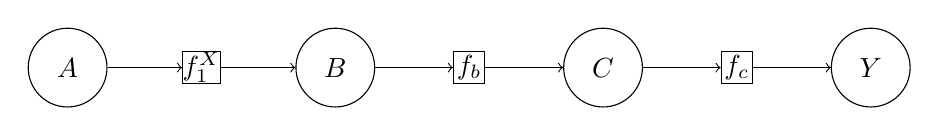
\begin{tikzpicture}[every place/.style={minimum size=10mm}, node distance=1.7cm]
  % Places
  \node[place] (A) {$A$};
  \node[transition] (fa) [right of=A] {$f_1^X$};
  \node[place] (B) [right of=fa] {$B$};
  \node[transition] (fb) [right of=B] {$f_b$};
  \node[place] (C) [right of=fb] {$C$};
  \node[transition] (fc) [right of=C] {$f_c$};
  \node[place] (Y) [right of=fc] {$Y$};

  % Arcs
  \draw[->] (A) -- (fa);
  \draw[->] (fa) -- (B);
  \draw[->] (B) -- (fb);
  \draw[->] (fb) -- (C);
  \draw[->] (C) -- (fc);
  \draw[->] (fc) -- (Y);
\end{tikzpicture}}
\caption{Resized Linear Petri Net}
\label{fig:linear_petri_resized}
\end{figure}

% Second instance as a regular figure
\begin{figure}[htbp]
\centering
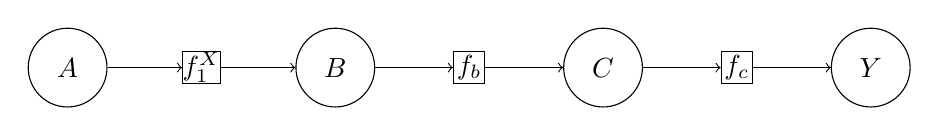
\begin{tikzpicture}[every place/.style={minimum size=10mm}, node distance=1.7cm]
  % Places
  \node[place] (A) {$A$};
  \node[transition] (fa) [right of=A] {$f_1^X$};
  \node[place] (B) [right of=fa] {$B$};
  \node[transition] (fb) [right of=B] {$f_b$};
  \node[place] (C) [right of=fb] {$C$};
  \node[transition] (fc) [right of=C] {$f_c$};
  \node[place] (Y) [right of=fc] {$Y$};

  % Arcs
  \draw[->] (A) -- (fa);
  \draw[->] (fa) -- (B);
  \draw[->] (B) -- (fb);
  \draw[->] (fb) -- (C);
  \draw[->] (C) -- (fc);
  \draw[->] (fc) -- (Y);
\end{tikzpicture}
\caption{Tensorized Petri Net Structure}
\label{fig:tensor_petri}
\end{figure}

\begin{figure}[htbp]
% Petri Net Model of the Producer-Consumer Problem (Refined)
\begin{tikzpicture}[node distance=2.2cm and 2.2cm, >=stealth, bend angle=30, auto, on grid]
    % Places
    \placewithtokens{producer}{0,0}{1}
    \placewithtokens{buffer}{2.8,0}{0}
    \placewithtokens{consumer}{5.6,0}{1}
    \placewithtokens{bufferCapacity}{2.8,-2.2}{3}

    % Transitions
    \node[transition, rounded corners=2pt] (produce) [right=of producer] {};
    \node[transition, rounded corners=2pt] (consume) [right=of buffer] {};

    % Arcs
    \draw[pre] (producer) -- (produce);
    \draw[post] (produce) -- (producer);
    \draw[post] (produce) -- (buffer);
    \draw[pre] (buffer) -- (consume);
    \draw[pre] (consumer) -- (consume);
    \draw[post] (consume) -- (consumer);
    \draw[pre] (bufferCapacity) -- (produce);
    \draw[post] (consume) -- (bufferCapacity);

    % Labels
    \node[above] at (producer.north) {Producer};
    \node[above] at (buffer.north) {Buffer};
    \node[above] at (consumer.north) {Consumer};
    \node[below] at (bufferCapacity.south) {Buffer Capacity};
    \node[above] at (produce.north) {Produce};
    \node[above] at (consume.north) {Consume};

    % Title
    \node[above=1cm] at (current bounding box.north) {Petri Net Model of the Producer-Consumer Problem};
\end{tikzpicture}
\caption{Producer-Consumer Workflow}
\label{fig:producer_consumer_workflow}
\end{figure}

\begin{figure}[htbp]
\centering
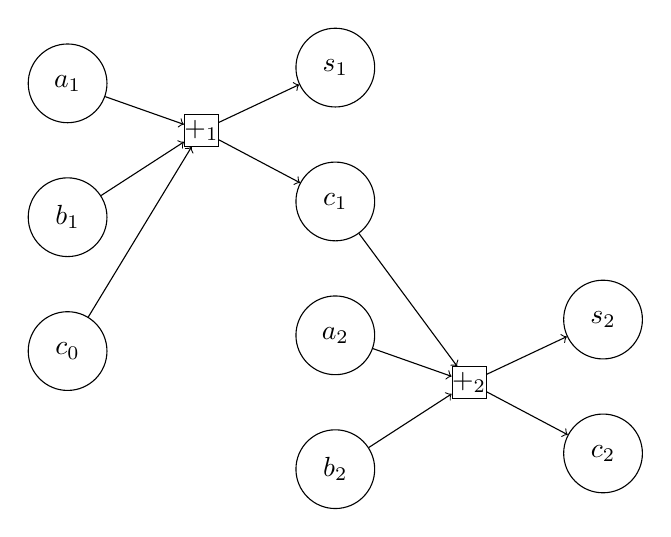
\begin{tikzpicture}[every place/.style={minimum size=10mm}, node distance=1.7cm and 2.2cm]
  % First digit addition
  \node[place] (a1) {$a_1$};
  \node[place, below of=a1] (b1) {$b_1$};
  \node[place, below of=b1] (c0) {$c_0$};
  \node[transition] (add1) [right of=b1, yshift=1.1cm] {$+_1$};
  \node[place] (s1) [right of=add1, yshift=0.8cm] {$s_1$};
  \node[place] (c1) [below of=s1] {$c_1$};

  \draw[->] (a1) -- (add1);
  \draw[->] (b1) -- (add1);
  \draw[->] (c0) -- (add1);
  \draw[->] (add1) -- (s1);
  \draw[->] (add1) -- (c1);

  % Second digit addition
  \node[place, below of=c1] (a2) {$a_2$};
  \node[place, below of=a2] (b2) {$b_2$};
  \node[transition] (add2) [right of=b2, yshift=1.1cm] {$+_2$};
  \node[place] (s2) [right of=add2, yshift=0.8cm] {$s_2$};
  \node[place] (c2) [below of=s2] {$c_2$};

  \draw[->] (a2) -- (add2);
  \draw[->] (b2) -- (add2);
  \draw[->] (c1) -- (add2);
  \draw[->] (add2) -- (s2);
  \draw[->] (add2) -- (c2);
\end{tikzpicture}
\caption{Carry Arithmetic as Feedback System.}
\label{fig:carry_arithmetic_feedback}
\end{figure}

\begin{figure}[htbp]
\centering
\resizebox{0.9\columnwidth}{!}{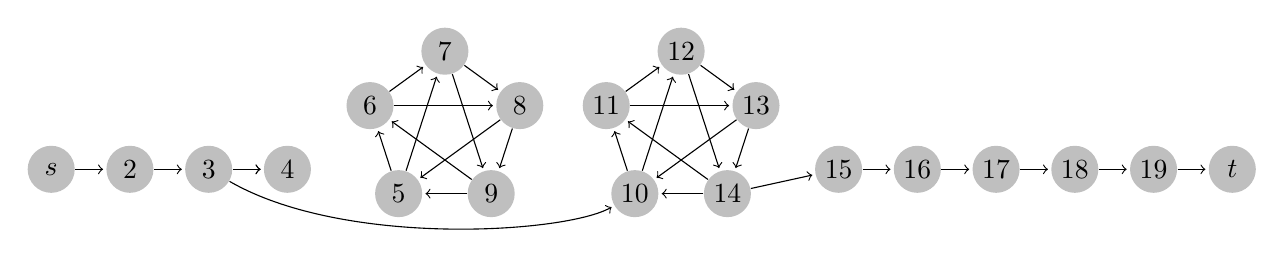
\begin{tikzpicture}
    [shorten >=1pt,->,
     vertex/.style={circle,fill=black!25,minimum size=17pt,inner sep=0pt}]
  
    \foreach \name/\x in {s/1, 2/2, 3/3, 4/4, 15/11, 16/12, 17/13, 18/14, 19/15, t/16}
      \node[vertex] (G-\name) at (\x,0) {$\name$};
  
    \foreach \name/\angle/\text in {P-1/234/5, P-2/162/6, P-3/90/7, P-4/18/8, P-5/-54/9}
      \node[vertex,xshift=6cm,yshift=.5cm] (\name) at (\angle:1cm) {$\text$};
  
    \foreach \name/\angle/\text in {Q-1/234/10, Q-2/162/11, Q-3/90/12, Q-4/18/13, Q-5/-54/14}
      \node[vertex,xshift=9cm,yshift=.5cm] (\name) at (\angle:1cm) {$\text$};
  
    \foreach \from/\to in {s/2,2/3,3/4,3/4,15/16,16/17,17/18,18/19,19/t}
      \draw (G-\from) -- (G-\to);
  
    \foreach \from/\to in {1/2,2/3,3/4,4/5,5/1,1/3,2/4,3/5,4/1,5/2}
      { \draw (P-\from) -- (P-\to); \draw (Q-\from) -- (Q-\to); }
  
    \draw (G-3) .. controls +(-30:2cm) and +(-150:1cm) .. (Q-1);
    \draw (Q-5) -- (G-15);
  \end{tikzpicture}}
\caption{Example of a complex graph structure with cycles and cross-connections.}
\label{fig:complex_graph_example}
\end{figure}

\subsection{Model Analysis}

To analyze the properties of our Petri Net model, we examine:

\begin{itemize}
    \item \textbf{Reachability}: Determining whether a specific marking can be reached from the initial marking.
    \item \textbf{Boundedness}: Ensuring that the number of tokens in each place does not exceed a finite bound.
    \item \textbf{Liveness}: Verifying that the model is free from deadlocks.
    \item \textbf{Fairness}: Ensuring that all enabled transitions eventually fire.
\end{itemize}

\subsection{Wiring Diagram Representation}

Figure \ref{fig:clock_with_display} presents a wiring diagram in the style of David Jaz Myers' work on Dynamical Systems, illustrating the structure of a clock system with display components.

\begin{figure}[htbp]
\centering
% ClockWithDisplay in Spivak/Fong style using oriented WD
\begin{tikzpicture}[oriented WD, bbx=1.2cm, bby=2ex, bb min width=2cm, bb port length=4pt, bb port sep=1.5]
    % Clock and Meridiem boxes with proper ports and more rounded corners
    % The notation bb={in}{out} specifies number of input and output ports
    \node[bb={0}{1}, fill=blue!15, thick, rounded corners=6pt] (clock) at (0, -2) {\footnotesize Clock};
    \node[bb={1}{1}, fill=blue!15, thick, rounded corners=6pt] (meridiem) at (0, 2) {\footnotesize Meridiem};
    
    % Container box that encompasses both components with more spacing
    \node[bb={0}{2}, fit={($(clock.south west)+(-0.8,-0.5)$) ($(meridiem.north east)+(0.8,0.5)$)}, thick] (container) {};
    
    % Connection from right of Clock to left of Meridiem
    % Symmetric S-curve for Clock→Meridiem (canonical categorical style)
    \draw
      (clock.east)
      .. controls ($(clock.east)+(2,2.8)$) and ($(meridiem.west)+(-2,-2.8)$)
      .. (meridiem.west);

    
    % Connect ports to container edges for outputs
    \draw (meridiem_out1) to (container_out1');
    \draw (clock_out1) to (container_out2');
    
    % External labels with better positioning
    \node[anchor=west, font=\footnotesize] at ($(container_out1)+(0.2,0)$) {a.m./p.m.};
    \node[anchor=west, font=\footnotesize] at ($(container_out2)+(0.2,0)$) {Hour};
    
    % Title below container with better spacing
    \node[font=\normalsize] at ($(container.south)+(0,0.5)$) {ClockWithDisplay};
\end{tikzpicture}
\caption{Wiring diagram of a clock with display components, showing the meridiem and hour display units.}
\label{fig:clock_with_display}
\end{figure}

\subsection{Implementation}

[Describe the tools or methods used to implement and analyze your Petri Net model]
\sectionheader{Results and Discussion}
\label{sec:results}

The Tensorized Petri Net formalism offers several advantages:

\begin{itemize}
    \item \textbf{Parallelism:} Tensor operations enable efficient, parallel updates of the Petri Net state, mirroring the inherent concurrency of the net.
    \item \textbf{Compositionality:} Polynomial functors provide a principled way to compose and decompose Petri Net modules, supporting scalable and reusable designs.
    \item \textbf{Interpretability:} The explicit representation of operands, operators, and their topological relationships makes the computation transparent and analyzable.
    \item \textbf{Expressiveness:} This framework generalizes naturally to other structured computations, such as cellular automata, graph algorithms, and symbolic reasoning tasks.
\end{itemize}

\subsection{Model Validation}

[Describe how you validated your Petri Net model]

\subsection{Performance Analysis}

[Present the results of your performance analysis]

\begin{table}[htbp]
\centering
\caption{Performance Metrics for Different Configurations}
\label{tab:performance}
\begin{tabular}{@{}lccc@{}}
\toprule
\textbf{Metric} & \textbf{Config 1} & \textbf{Config 2} & \textbf{Config 3} \\
\midrule
Throughput & [value] & [value] & [value] \\
Response Time & [value] & [value] & [value] \\
Resource Utilization & [value] & [value] & [value] \\
\bottomrule
\end{tabular}
\end{table}

\subsection{Case Study}

[Present a case study demonstrating the application of your Petri Net model]

\subsection{Discussion}

[Discuss the implications of your results and any limitations of your approach]

\begin{figure}[htbp]
\centering
\resizebox{0.9\columnwidth}{!}{% Petri Net Model of the Producer-Consumer Problem (Refined)
\begin{tikzpicture}[node distance=2.2cm and 2.2cm, >=stealth, bend angle=30, auto, on grid]
    % Places
    \placewithtokens{producer}{0,0}{1}
    \placewithtokens{buffer}{2.8,0}{0}
    \placewithtokens{consumer}{5.6,0}{1}
    \placewithtokens{bufferCapacity}{2.8,-2.2}{3}

    % Transitions
    \node[transition, rounded corners=2pt] (produce) [right=of producer] {};
    \node[transition, rounded corners=2pt] (consume) [right=of buffer] {};

    % Arcs
    \draw[pre] (producer) -- (produce);
    \draw[post] (produce) -- (producer);
    \draw[post] (produce) -- (buffer);
    \draw[pre] (buffer) -- (consume);
    \draw[pre] (consumer) -- (consume);
    \draw[post] (consume) -- (consumer);
    \draw[pre] (bufferCapacity) -- (produce);
    \draw[post] (consume) -- (bufferCapacity);

    % Labels
    \node[above] at (producer.north) {Producer};
    \node[above] at (buffer.north) {Buffer};
    \node[above] at (consumer.north) {Consumer};
    \node[below] at (bufferCapacity.south) {Buffer Capacity};
    \node[above] at (produce.north) {Produce};
    \node[above] at (consume.north) {Consume};

    % Title
    \node[above=1cm] at (current bounding box.north) {Petri Net Model of the Producer-Consumer Problem};
\end{tikzpicture}}
\caption{Producer-Consumer Workflow Analysis}
\label{fig:producer_consumer}
\end{figure}
\paragraph{Cultural and Historical Context: Ethno Arithmetic and Fractal Patterns}

The GASing method finds profound resonance with the work of Professor Ron Eglash on \textbf{Ethno Arithmetic} and fractal patterns in Indigenous knowledge systems. Eglash's research (Eglash, 1999) demonstrates how many African, Native American, and other Indigenous cultures developed sophisticated mathematical concepts through fractal patterns in their art, architecture, and social organizations. These patterns, often embedded in cultural practices, represent an early form of \textbf{progressive function application} and \textbf{self-similar computation} that predates Western formal mathematics.

GASing's digit-wise, cell-like modules parallel the recursive, self-similar structures found in Indigenous fractal designs, where complex patterns emerge from the repeated application of simple rules—a principle that mirrors GASing's approach to arithmetic through the progressive application of addition. The \textbf{combinatorial patterns} in GASing's digit-wise processing echo the recursive geometric transformations observed in African fractals, where simple scaling rules generate complex, computationally rich structures.

This connection is particularly significant because it suggests that GASing's approach is not merely a technical innovation but part of a broader human tradition of pattern-based computation. By recognizing these parallels, GASing bridges modern computational thinking with historical mathematical practices, creating a more inclusive framework that honors diverse mathematical traditions while providing a foundation for future computational paradigms.
\paragraph{Computational Foundations}

The GASing arithmetic method positions the foundational architecture of computing tasks by elevating addition to the role of meta-operator—a universal primitive from which all arithmetic logic operations can be systematically constructed, analyzed, and verified. This reductionist approach is not merely a theoretical exercise; it provides a practical, measurable framework for assessing resource consumption, numerical precision, and logical correctness in both human and machine reasoning. As modern LLM technologies have conclusively demonstrated, even \textbf{the most sophisticated reasoning and content generation processes}—from poetry composition to mathematical proof generation—\textbf{can be carried out with arithmetic operations} as their fundamental computational substrate. The seemingly magical capabilities of these systems emerge entirely from operations that, at their core, are nothing more than carefully orchestrated \textbf{patterns of addition and multiplication}.

By \textbf{conceptually decomposing} complex operations such as multiplication, subtraction, and division into sequences of segment-wise additions, GASing enables explicit quantification of computational effort: every operation is traceable to a countable set of addition-equivalent steps. This transparency allows for rigorous evaluation and optimization of both cognitive and computational resource usage, offering a clear metric for comparing algorithms, implementations, or even reasoning strategies. Such granularity is invaluable for designing systems—human or artificial—that must operate within strict resource constraints, whether those are working memory, processing time, or energy consumption.

GASing’s focus on addition as the core operator also underpins a unified, cross-referential decision framework. By expressing all arithmetic logic in terms of addition, the method ensures that every step is both interpretable and verifiable, supporting robust provenance tracking and error detection. This unification bridges symbolic and sub-symbolic computation, aligning the clarity of rule-based logic with the efficiency of neural and matrix-based operations. The result is a system where numerical precision and logical correctness are not competing priorities, but mutually reinforcing outcomes of a single, transparent process.

Originally conceived to accelerate arithmetic calculation and reduce cognitive load for learners, GASing’s segment-wise, pattern-driven approach is grounded in well-established cognitive principles, such as chunking and resource preservation. It empowers users to adapt the granularity of operations to their own cognitive limits, minimizing mental effort while maximizing accuracy and speed. This adaptability is mirrored in modern AI, where resource management and interpretability are critical for scaling intelligent systems.

In summary, GASing arithmetic is more than a pedagogical innovation—it is a rigorous, interpretable, and scalable substrate for reasoning that bridges the gap between human cognition and machine computation. By grounding all operations in addition, GASing delivers a framework where every logical step is measurable, every result is verifiable, and every computation is optimized for resource efficiency.

At a deeper level, GASing establishes \textbf{\textbf{\textit{addition}}} as a universal atomic "token" of computational effort—a fundamental unit of measure that enables precise resource accounting across all computational contexts, from silicon chips to human minds. This resource-aware arithmetic framework redefines how we attribute and measure cognitive and computational work, creating a unified currency of effort that makes the cost of any reasoning process explicitly quantifiable. Each "adding action" becomes a credit unit within a universal ledger of computational activity, allowing systems to track, allocate, and optimize resources with unprecedented granularity. This approach transcends traditional hardware-specific metrics (like CPU cycles or memory usage) to establish a hardware-agnostic measure of fundamental reasoning operations.

This philosophical reinterpretation of what counting fundamentally means represents a major advancement in how we conceptualize and accumulate knowledge about the world. By establishing the addition operation as the atomic unit of reasoning, GASing provides a common denominator for measuring all forms of information processing, creating a bridge between disparate computational paradigms—quantum, neural, symbolic—and human cognition. It enables precise verification chains that can track not just the results of computation, but the exact resource cost of arriving at those results, providing a meta-level framework for reasoning about reasoning itself.

Intellectually, grounding all computational tasks in a single unifying operator yields an additional, profound benefit: it encourages both human and machine minds to converge on a shared pattern of reasoning. This shared pattern not only accumulates experience and impressions, but also aligns prior intentions and fosters deeper mutual understanding. In the abstract, aligning minds—whether individual, collective, or artificial—around a common operator is a necessary condition for establishing a unified theory of learning. Only by sharing such a foundational operator can human, machine, or organizational learning truly converge on a common framework, enabling the transfer and accumulation of knowledge, experience, and intention across all forms of intelligence.

As AI systems become increasingly autonomous and integrated into human workflows, such foundational clarity and measurability will be essential for ensuring trust, transparency, and continual improvement in both artificial and human intelligence. Modern LLMs have definitively proven that even the most advanced cognitive-seeming tasks—from multimodal reasoning to creative problem-solving—ultimately resolve to sequences of arithmetic operations. This revelation means that optimizing these fundamental operations is not merely an engineering detail but a strategic imperative with cascading benefits for AI capabilities, energy consumption, and accessibility. By \textbf{minimizing the resource footprint of these basic arithmetic operations through the principles outlined in GASing}, we can achieve dramatic improvements in these proven useful and pragmatic AI applications regardless of their apparent complexity or sophistication.

\textbf{Crucially, by grounding AI-powered reasoning in well-documented and human-understandable conceptual abstractions, GASing eliminates dependencies on specific hardware or software implementations.} The correctness verification process can always be traced back to the axiomatic definition of addition and the finite vocabulary admitted in each application context. This creates an adaptive yet fundamentally terminable reasoning framework—one that can evolve with technological advances without losing its verifiability. As hardware implementations evolve from classical computing to neuromorphic processors or quantum computers, the GASing verification mechanisms remain stable and interpretable to humans because they depend on mathematical properties, not implementation details. This ensures a consistent standard of correctness while enabling continuous innovation in the underlying technologies.

GASing's commitment to a minimal, interpretable operational vocabulary thus stands as both a practical solution and a philosophical imperative for the future of collaborative reasoning—one where the economics of knowledge acquisition can be precisely quantified, compared, and optimized across the full spectrum of computational agents, from the simplest calculator to the most sophisticated AI system to the human mind itself.

\bibliographystyle{plain}
\bibliography{bibliography}

\end{document}